\section{واحد کنترل (\lr{Control Unit}) و ماشین حالت (\lr{FSM})}
واحد کنترل به صورت یک ماشین حالت سنکرون (\lr{Synchronous FSM}) طراحی شده است که وظیفه مدیریت مراحل مختلف محاسبه و تولید سیگنال‌های کنترلی مسیر داده (\lr{Datapath}) را بر عهده دارد. این واحد شامل یک رجیستر ۳ بیتی برای ذخیره‌سازی حالت فعلی، یک رمزگشای $3 \to 8$ (\lr{Decoder}) برای تولید سیگنال یکتای هر حالت، و منطق ترکیبی برای محاسبه حالت بعدی (\lr{Next-State Logic}) است. ماشین حالت طراحی شده دارای ۷ حالت معتبر است که جزئیات کاربرد و کدگذاری مختصر آن‌ها در جدول زیر آمده است.

\begin{table}[H]
    \centering
    \caption{کدگذاری و وظایف حالت‌های ماشین کنترل}
    \vspace{0.2cm}
    \begin{tabular}{|c|c|c|}
        \hline
        \textbf{حالت}         & \textbf{کد باینری} & \textbf{شرح مختصر عملکرد در مدار}                          \\
        \hline
        \lr{\code{IDLE}}      & $000$              & انتظار برای فعال شدن سیگنال \lr{\code{Start}}              \\
        \hline
        \lr{\code{UNPACK}}    & $001$              & تفکیک فیلدها و بارگذاری رجیسترهای اولیه                    \\
        \hline
        \lr{\code{ALIGN}}     & $010$              & هم‌ارزش‌سازی نماها با شیفت مانتیس عدد کوچک‌تر                 \\
        \hline
        \lr{\code{ADD}}       & $011$              & انجام عملیات جمع یا تفریق کسرها توسط \lr{\code{Big\_ALU}}  \\
        \hline
        \lr{\code{NORMALIZE}} & $100$              & اصلاح گام‌به‌gام نما و مانتیس تا رسیدن به فرم استاندارد      \\
        \hline
        \lr{\code{ROUND}}     & $101$              & گرد کردن کسر نهایی بر اساس منطق \lr{Round-to-Nearest-Even} \\
        \hline
        \lr{\code{DONE}}      & $110$              & اعلام پایان محاسبات و تثبیت خروجی نهایی                    \\
        \hline
    \end{tabular}
\end{table}

منطق انتقال حالت بر اساس فلوچارت الگوریتم و سیگنال‌های فیدبک مسیر داده پیاده‌سازی شده است. ورودی‌های رجیستر حالت به کمک یک تفکیک‌کننده (\lr{Splitter}) مجزا شده‌اند و مقدار هر بیت حالت بعدی توسط گیت‌های ترکیبی بر اساس جدول انتقال حالت زیر مشخص می‌گردد.

\begin{table}[H]
    \centering
    \caption{جدول انتقال حالت ماشین کنترل (\lr{State Transition Table})}
    \vspace{0.2cm}
    \begin{tabular}{|c|c|c|}
        \hline
        \textbf{حالت فعلی}                     & \textbf{شرط انتقال}                                                         & \textbf{حالت بعدی}    \\
        \hline
        \lr{\code{IDLE}}                       & $\text{\lr{\code{Start}}} = 1$                                              & \lr{\code{UNPACK}}    \\
        \hline
        \lr{\code{UNPACK}}                     & —                                                                           & \lr{\code{ALIGN}}     \\
        \hline
        \lr{\code{ALIGN}}                      & —                                                                           & \lr{\code{ADD}}       \\
        \hline
        \lr{\code{ADD}}                        & —                                                                           & \lr{\code{NORMALIZE}} \\
        \hline
        \multirow{3}{*}{\lr{\code{NORMALIZE}}} & $\text{\lr{\code{need\_right}}} = 1 \lor \text{\lr{\code{need\_left}}} = 1$ & \lr{\code{NORMALIZE}} \\
        \cline{2-3}
                                               & $\text{\lr{\code{exception}}} = 1$                                          & \lr{\code{DONE}}      \\
        \cline{2-3}
                                               & \text{نرمال شدن مانتیس}                                                     & \lr{\code{ROUND}}     \\
        \hline
        \multirow{2}{*}{\lr{\code{ROUND}}}     & $\text{\lr{\code{round\_unnorm}}} = 1$                                      & \lr{\code{NORMALIZE}} \\
        \cline{2-3}
                                               & $\text{\lr{\code{round\_unnorm}}} = 0$                                      & \lr{\code{DONE}}      \\
        \hline
        \multirow{2}{*}{\lr{\code{DONE}}}      & $\text{\lr{\code{Start}}} = 0$                                              & \lr{\code{DONE}}      \\
        \cline{2-3}
                                               & $\text{\lr{\code{Start}}} = 1$                                              & \lr{\code{UNPACK}}    \\
        \hline
    \end{tabular}
\end{table}

سیگنال‌های کنترلی مورد نیاز در مسیر داده نیز به صورت کاملاً ترکیبی و صرفاً با تجمیع سیگنال‌های خروجی رمزگشا تولید می‌شوند. ساختار سخت‌افزاری واحد کنترل در شکل زیر نشان داده شده است.

\begin{figure}[H]
    \centering
    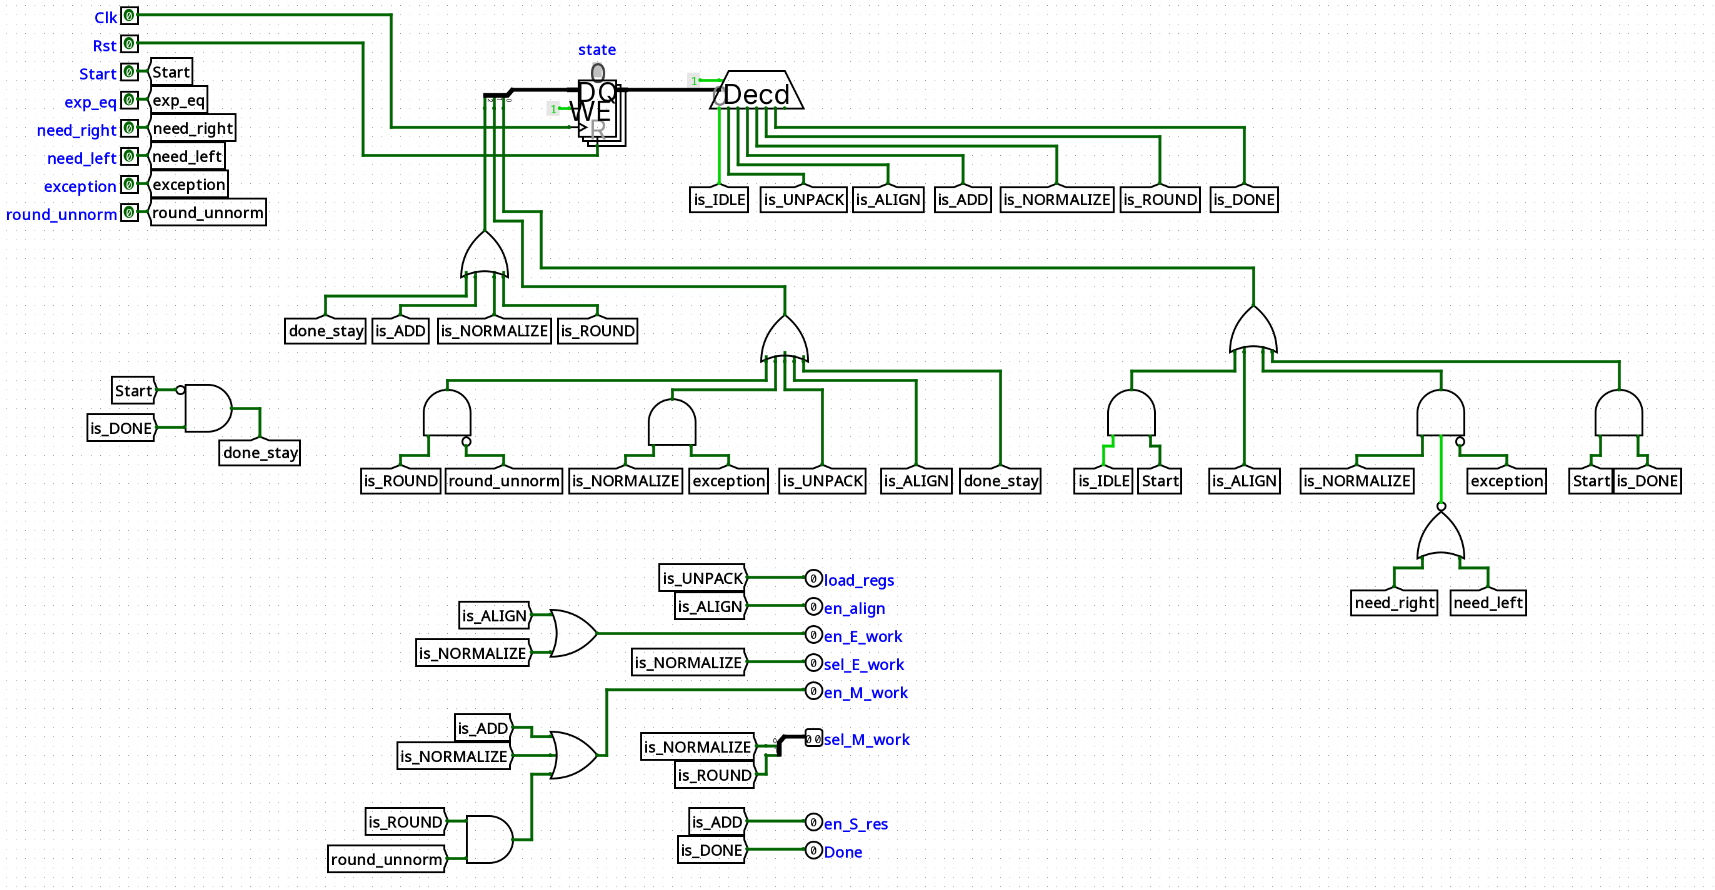
\includegraphics[width=1.0\textwidth]{assets/ctrl_unit.png}
    \caption{مدار سخت‌افزاری واحد کنترل (\lr{\code{Ctrl\_Unit}}) در محیط لاجیسیم}
\end{figure}

\pagebreak

\section{توصیف زیرمدارها}
در این بخش، ساختار و منطق پیاده‌سازی زیرمدارهای اصلی که مسیر داده (\lr{Datapath}) سیستم ممیز شناور را تشکیل می‌دهند، بررسی می‌شود.

\subsection{ماژول مقایسه و تفاضل نماها (\lr{\code{Exp\_Sub}})}
این ماژول وظیفه محاسبه اختلاف نماها و تعیین نمای بزرگ‌تر جهت هم‌ارزش‌سازی را بر عهده دارد. برای این منظور، از دو تفریق‌کننده موازی استفاده شده است که به‌طور هم‌زمان مقادیر $\text{\lr{\code{Ea}}} - \text{\lr{\code{Eb}}}$ و $\text{\lr{\code{Eb}}} - \text{\lr{\code{Ea}}}$ را محاسبه می‌کنند. سیگنال انتخاب‌گرِ (\lr{Select}) یک مالتی‌پلکسر مستقیماً به خروجیِ یک مقایسه‌کننده ($\text{\lr{\code{Ea}}} > \text{\lr{\code{Eb}}}$) متصل شده است تا همواره تفاضل مثبت را به عنوان خروجی (\lr{\code{diff}}) برگزیند. همچنین سیگنال وضعیت $\text{\lr{\code{a\_larger}}}$ با اعمال یک گیت \lr{\code{NOT}} بر روی خروجی مقایسه‌کننده تولید می‌شود.

\begin{figure}[H]
    \centering
    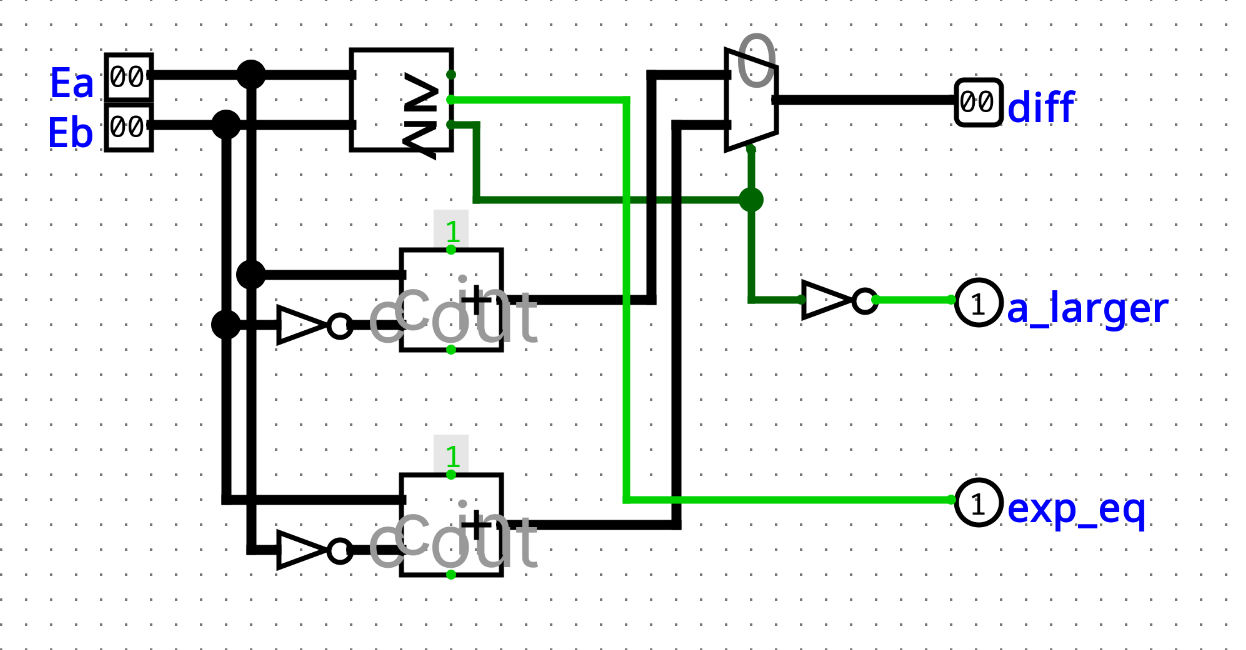
\includegraphics[width=0.7\textwidth]{assets/exp_sub.png}
    \caption{مدار داخلی ماژول \lr{\code{Exp\_Sub}}}
\end{figure}

\subsection{ماژول شیفت‌دهنده مانتیس (\lr{\code{Mantissa\_Shift}})}
این واحد وظیفه شیفت به راستِ مانتیس عددِ کوچک‌تر را برای برابر شدن نماها بر عهده دارد. داده‌ها ابتدا به ۳۲ بیت بسط داده شده و پس از عبور از یک شیفت‌دهنده بشکه‌ای (\lr{Barrel Shifter})، با استفاده از ابزار \lr{\code{Splitter}} تنها بیت‌های 0 تا 26 (۲۷ بیت کم‌ارزش) به عنوان خروجی استخراج شده و بیت‌های اضافی دور ریخته می‌شوند. برای مدیریت شیفت‌های بزرگ‌تر از ۲۷ (که مانتیس را کاملاً صفر می‌کنند)، از یک مقایسه‌کننده برای بررسی شرط $\text{\lr{\code{Shift\_Amt}}} < 17$ استفاده شده است. خروجی این شرط مشخص می‌کند که مالتی‌پلکسرِ نهایی، مقدار شیفت‌یافته را عبور دهد یا آن را با مقدار ثابت صفر جایگزین کند.

\begin{figure}[H]
    \centering
    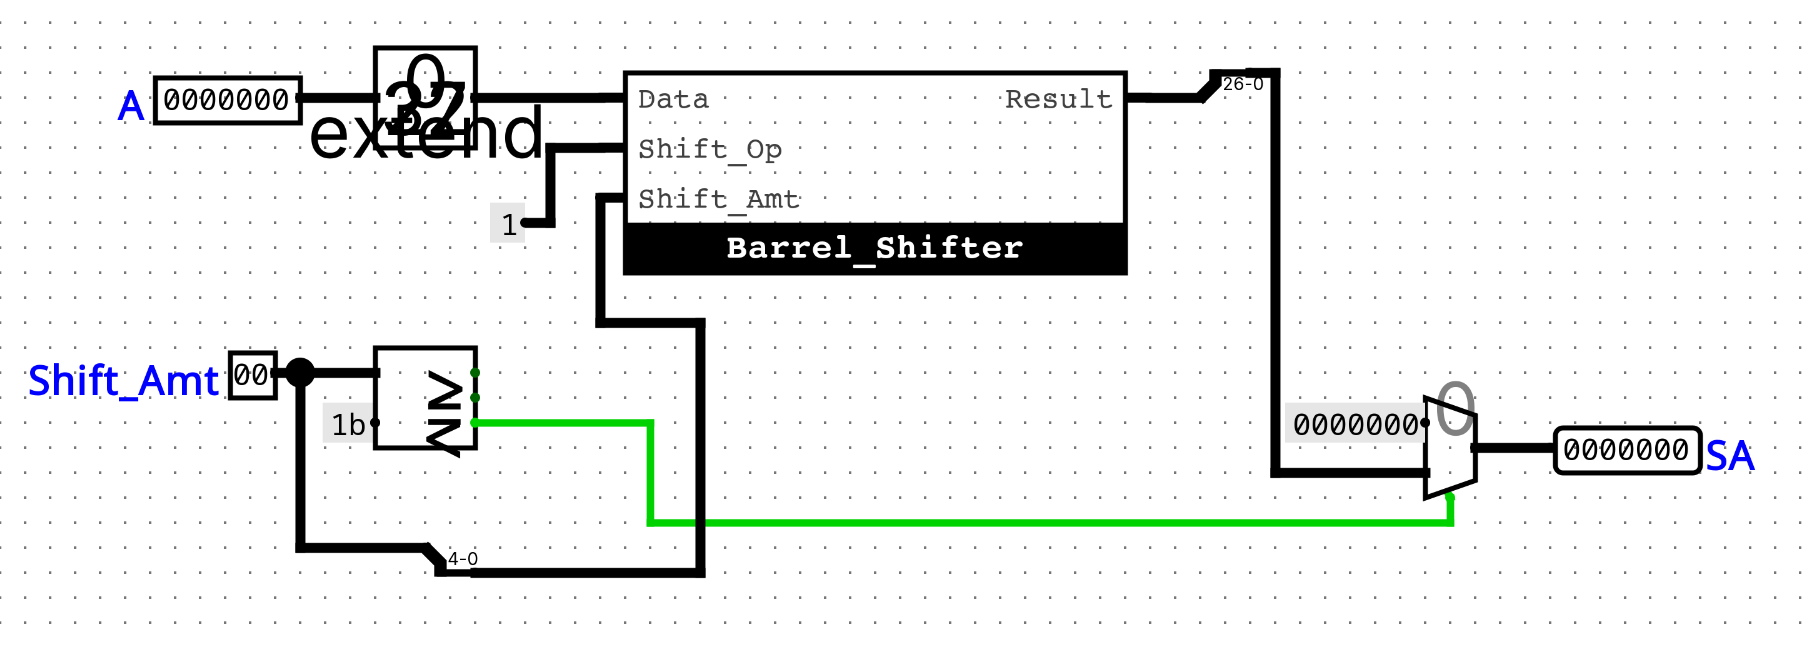
\includegraphics[width=0.8\textwidth]{assets/mantissa_shift.png}
    \caption{مدار داخلی ماژول \lr{\code{Mantissa\_Shift}}}
\end{figure}

\subsection{ماژول محاسبه‌گر اصلی (\lr{\code{Big\_ALU}})}
این ماژول عملیات اصلی جمع یا تفریق کسرها را با مدیریت صحیح علامت‌ها انجام می‌دهد. برای بخش تفریق، مشابه استراتژی بخش نما، دو تفریق‌کننده موازی مقادیر $\text{\lr{\code{Ma}}} - \text{\lr{\code{Mb}}}$ و $\text{\lr{\code{Mb}}} - \text{\lr{\code{Ma}}}$ را تولید کرده و یک مالتی‌پلکسر، نتیجه مثبت را انتخاب می‌کند. سپس یک مالتی‌پلکسر دیگر بر اساس نوع عملیات درخواستی (که از بررسی علامت‌ها و سیگنال \lr{\code{Sub}} به دست می‌آید)، خروجی نهایی را بین حاصل‌جمع ($\text{\lr{\code{Ma}}} + \text{\lr{\code{Mb}}}$) و تفاضلِ مثبت انتخاب می‌کند.

\begin{figure}[H]
    \centering
    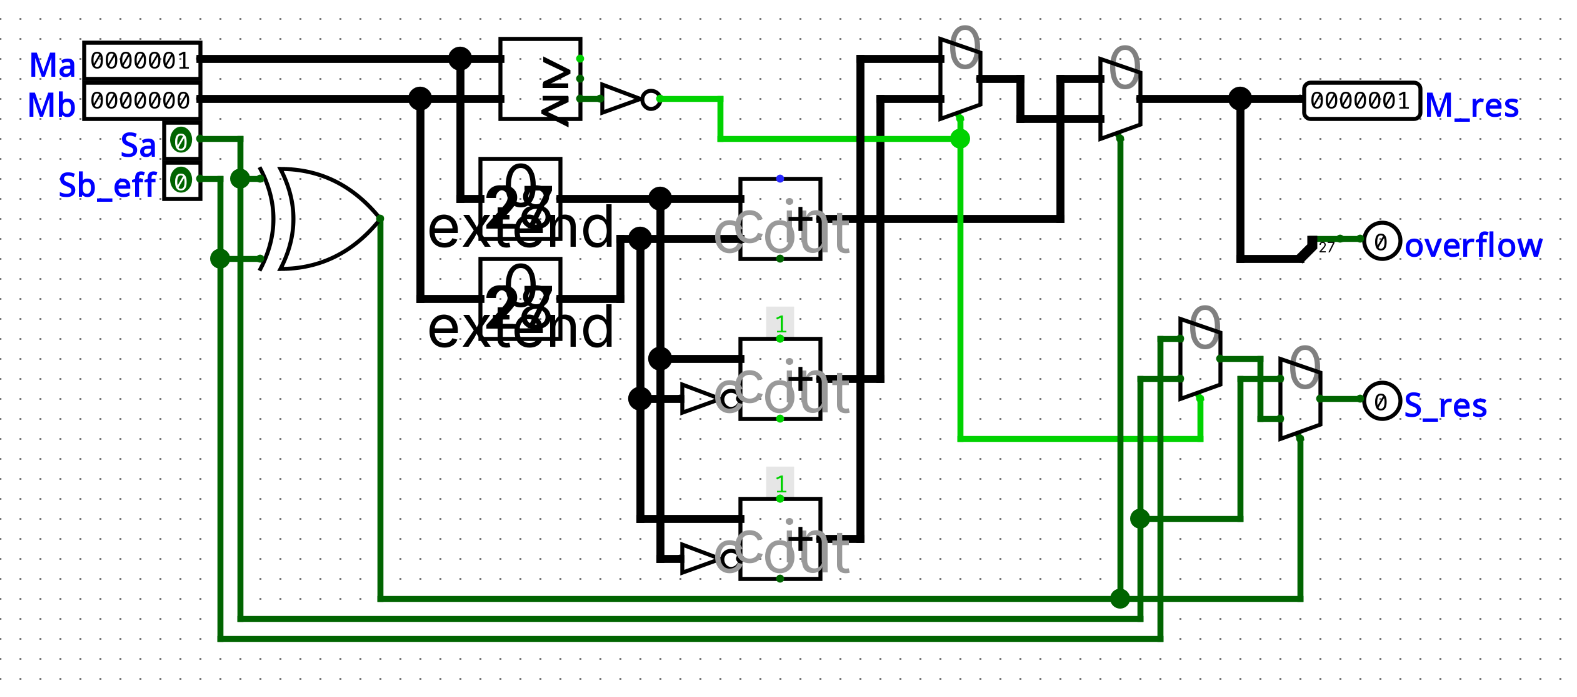
\includegraphics[width=0.8\textwidth]{assets/big_alu.png}
    \caption{مدار داخلی ماژول \lr{\code{Big\_ALU}}}
\end{figure}

\subsection{ماژول نرمال‌سازی (\lr{\code{Normalizer}})}
این واحد در هر چرخه ساعت یک گام نرمال‌سازی (به راست یا چپ) را روی کسر اعمال می‌کند. سیگنال‌های کنترلیِ نرمال‌سازی به صورت ترکیبی از روی مانتیس و نمای ورودی استخراج می‌شوند. سیگنال نیاز به شیفت به راست (\lr{\code{need\_right}}) مستقیماً به بیت سرریز کسر یعنی $\text{\lr{\code{M\_in[27]}}}$ متصل است. تشخیص نیاز به شیفت به چپ (\lr{\code{need\_left}}) نیز با بررسی وجود صفر پیشتاز و غیرصفر بودن نما، از طریق رابطه منطقی زیر به دست می‌آید:
\begin{align*}
    \text{\lr{\code{need\_left}}} = \overline{\text{\lr{\code{M\_in[27]}}}} \cdot \overline{\text{\lr{\code{M\_in[26]}}}} \cdot (\text{\lr{\code{E\_in}}} > 0)
\end{align*}

\begin{figure}[H]
    \centering
    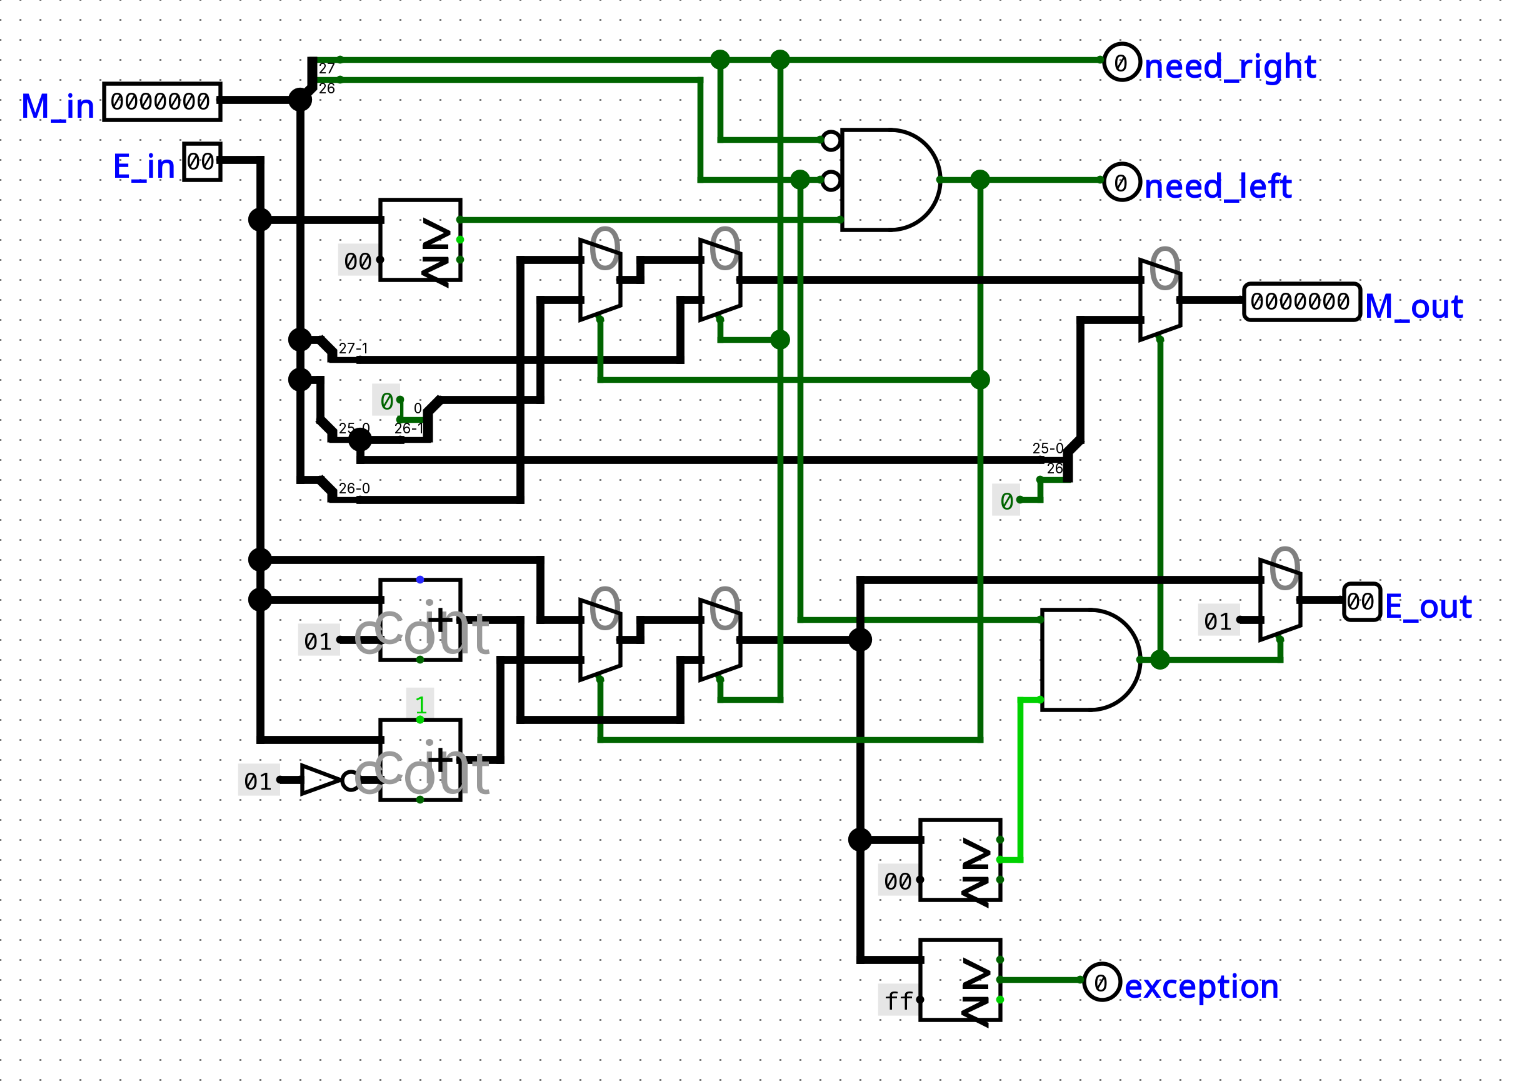
\includegraphics[width=0.7\textwidth]{assets/normalizer.png}
    \caption{مدار داخلی ماژول \lr{\code{Normalizer}}}
\end{figure}

\subsection{ماژول گرد کردن (\lr{\code{Rounder}})}
این ماژول با پیاده‌سازی منطق استاندارد \lr{Round-to-Nearest-Even}، کسر ۲۷ بیتی را به ۲۳ بیت نهایی تقلیل می‌دهد. تصمیم‌گیری برای گرد کردن به بالا (افزودن یک واحد) با بررسی بیت‌های محافظ (\lr{\code{M\_in[2]}})، گرد کردن (\lr{\code{M\_in[1]}})، چسبنده (\lr{\code{M\_in[0]}}) و کم‌ارزش‌ترین بیتِ کسر (\lr{\code{M\_in[3]}}) انجام می‌پذیرد. این شرط به‌صورت ترکیبی محاسبه شده و به پایه \lr{\code{Carry-in}} یک جمع‌کننده که وظیفه جمع کسر با صفر را دارد، متصل می‌شود:
\begin{align*}
    \text{\lr{\code{Carry\_in}}} = \text{\lr{\code{M\_in[2]}}} \cdot (\text{\lr{\code{M\_in[1]}}} \lor \text{\lr{\code{M\_in[0]}}} \lor \text{\lr{\code{M\_in[3]}}})
\end{align*}
در صورتی که عملیات گرد کردن به بالا منجر به سرریز مجدد کسر شود، بیت ۲۷ اُم خروجیِ جمع‌کننده، سیگنال $\text{\lr{\code{round\_unnorm}}} = 1$ را فعال می‌کند تا ماشین حالت مجدداً به وضعیت نرمال‌سازی بازگردد.

\begin{figure}[H]
    \centering
    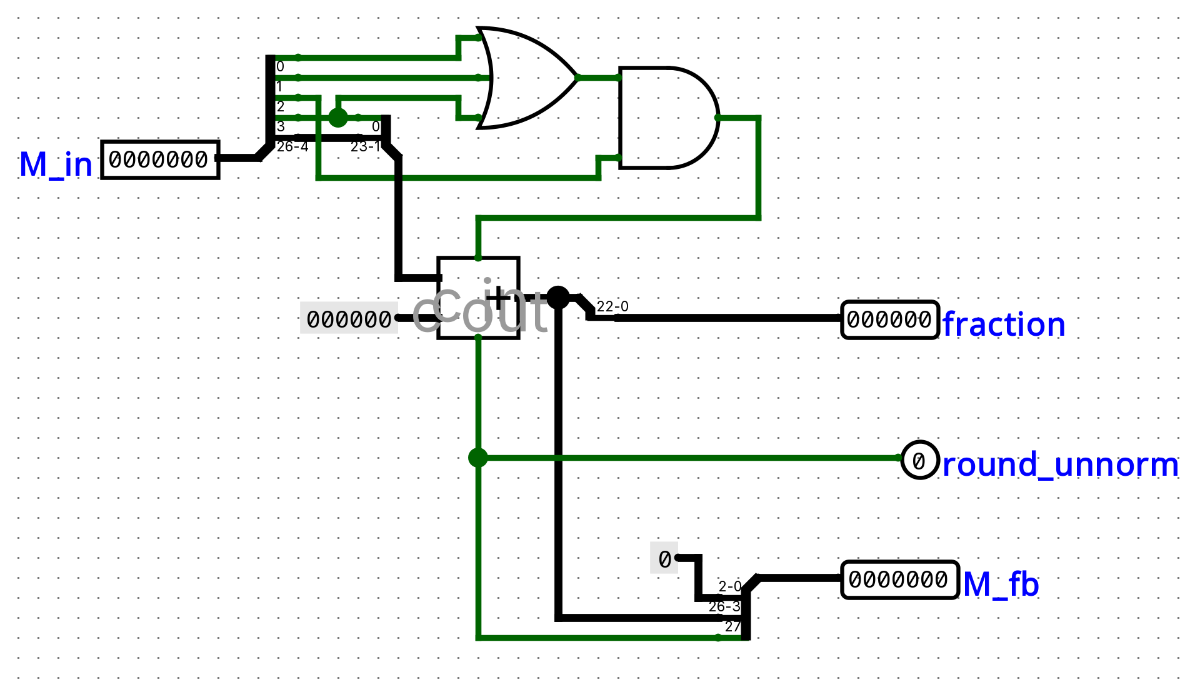
\includegraphics[width=0.8\textwidth]{assets/rounder.png}
    \caption{مدار داخلی ماژول \lr{\code{Rounder}}}
\end{figure}

\pagebreak

\section{مسیر داده (\lr{Datapath})}
مسیر داده وظیفه ذخیره‌سازی موقت داده‌ها، تفکیک فیلدها و هدایت آن‌ها به سمت واحدهای محاسباتی را بر عهده دارد. اجزای اصلی تشکیل‌دهنده این بخش شامل زیرمدارهای توصیف‌شده و مجموعه‌ای از رجیسترها شامل $\text{\lr{\code{Sa\_reg}}}$، $\text{\lr{\code{Sb\_eff\_reg}}}$، رجیسترهای نما $\text{\lr{\code{Ea\_reg}}}$ و $\text{\lr{\code{Eb\_reg}}}$، رجیسترهای مانتیس اولیه $\text{\lr{\code{Ma\_reg}}}$ و $\text{\lr{\code{Mb\_reg}}}$، و رجیسترهای کاری $\text{\lr{\code{E\_work\_reg}}}$، $\text{\lr{\code{M\_work\_reg}}}$ و $\text{\lr{\code{S\_res\_reg}}}$ است که همگی با سیگنال سنکرون \lr{\code{Rst}} بازنشانی می‌شوند.

در مرحله تفکیک فیلدها (\lr{Unpack})، بیت پنهان (\lr{Hidden bit}) برای هر دو ورودی با بررسی شرط غیرصفر بودن نما ($\text{\lr{\code{exp}}} \neq 0$) به کمک مقایسه‌کننده و گیت \lr{\code{NOT}} تولید شده و به پشت کسر چسبانده می‌شود. همچنین ۳ بیت صفر نیز به عنوان بیت‌های \lr{GRS} به سمت راست کسرها متصل می‌گردند تا مانتیس‌های اولیه ۲۷ بیتی شکل بگیرند.

بیت علامت مؤثر عملوند دوم از رابطه منطقی $\text{\lr{\code{B[31]}}} \oplus \text{\lr{\code{Sub}}}$ محاسبه شده و در رجیستر $\text{\lr{\code{Sb\_eff\_reg}}}$ ذخیره می‌شود تا خروجی آن مستقیماً به ورودی ماژول \lr{\code{Big\_ALU}} هدایت گردد.

خروجی ۳۲ بیتی نهایی (\lr{\code{Result}}) فاقد رجیستر خروجی اختصاصی است و به صورت ترکیبی از کنار هم قرار گرفتن فیلدهای نهایی ساخته می‌شود؛ بنابراین مقدار این کلمه خروجی تنها در زمان فعال بودن سیگنال $\text{\lr{\code{Done}}} = 1$ معتبر و قابل استناد خواهد بود. ساختار اتصالات مسیر داده در شکل زیر آورده شده است.

\begin{figure}[H]
    \centering
    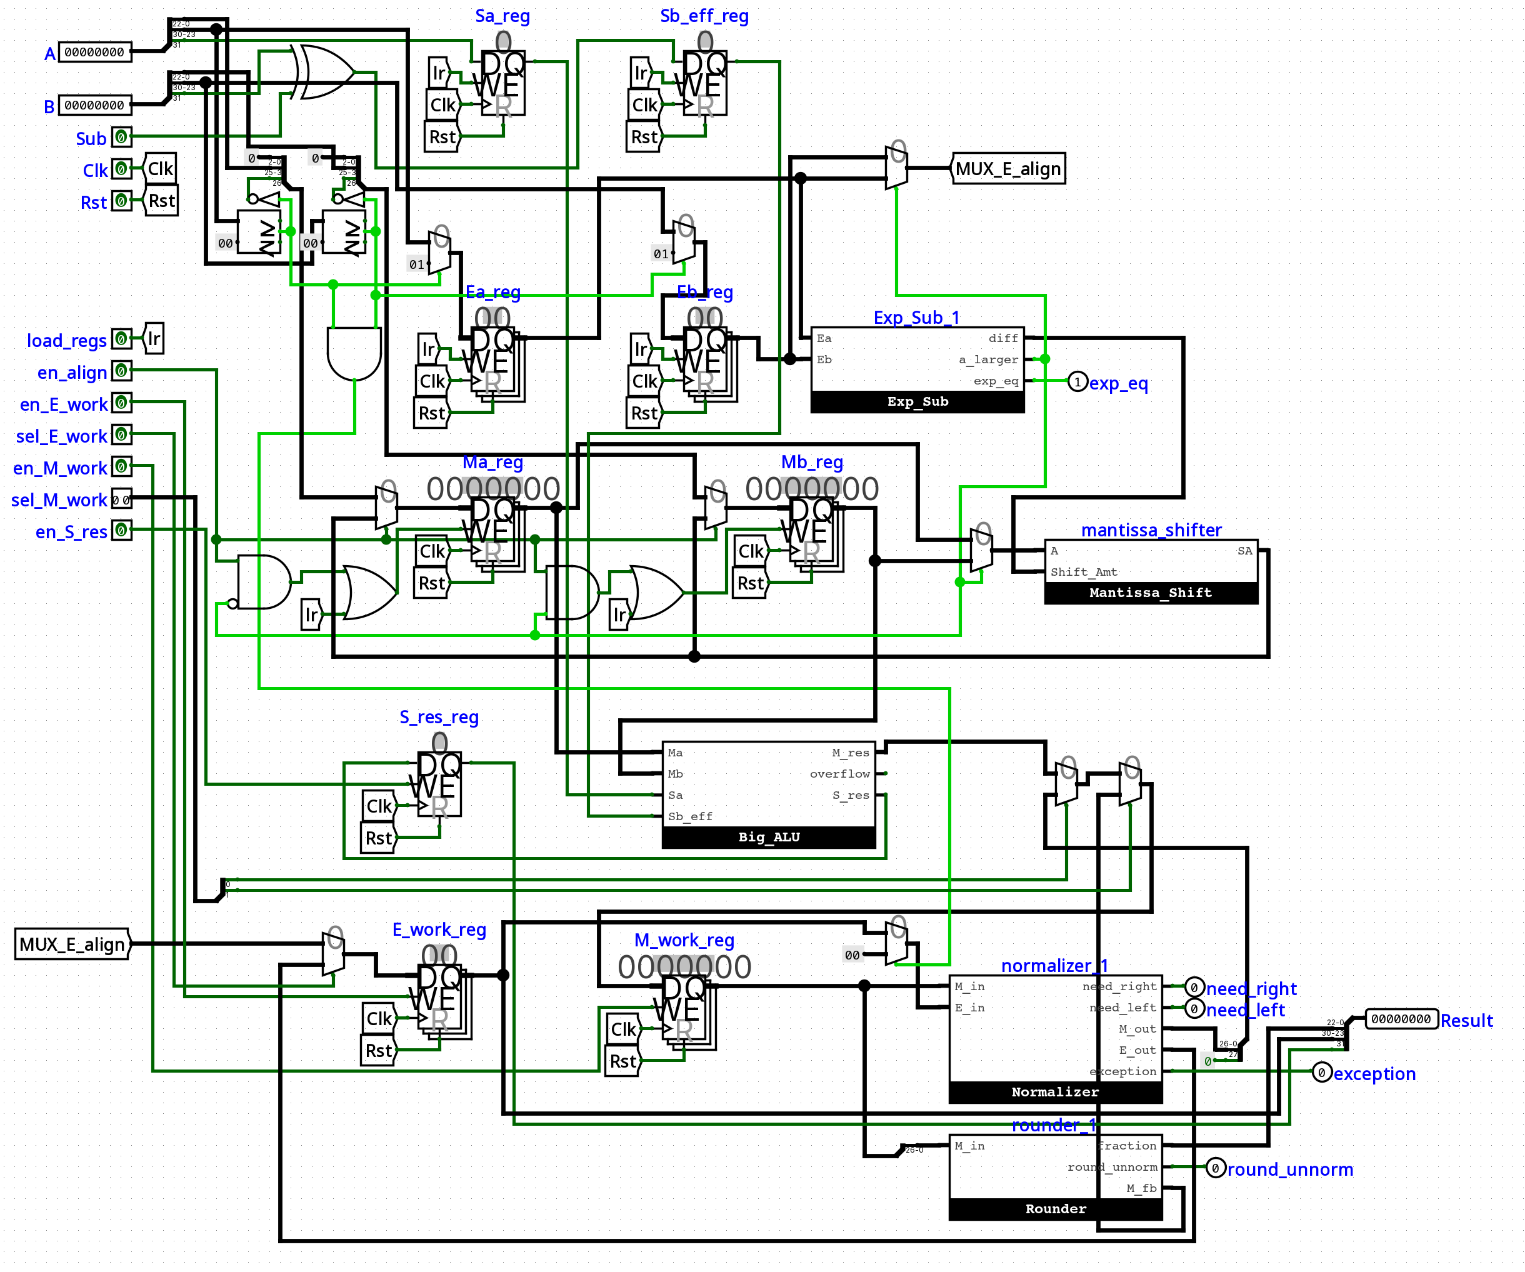
\includegraphics[width=1.0\textwidth]{assets/datapath.png}
    \caption{نمای کلی مدار مسیر داده (\lr{Datapath}) در محیط لاجیسیم}
\end{figure}

\pagebreak

\section{مدار سطح بالا (\lr{Top-Level})}
در ماژول اصلی (\lr{\code{main}})، واحد کنترل (\lr{\code{Ctrl\_Unit}}) و مسیر داده (\lr{\code{Datapath}}) به یکدیگر متصل شده‌اند تا سیستم کامل جمع و تفریق‌کننده ممیز شناور شکل بگیرد. این ماژول دارای ۶ ورودی شامل داده‌های ۳۲ بیتی $\text{\lr{\code{A}}}$ و $\text{\lr{\code{B}}}$، سیگنال‌های کنترلی تک‌بیتی $\text{\lr{\code{Sub}}}$، $\text{\lr{\code{Clk}}}$، $\text{\lr{\code{Rst}}}$ و $\text{\lr{\code{Start}}}$، و همچنین ۲ خروجی شامل حاصل نهایی ۳۲ بیتی $\text{\lr{\code{Result}}}$ و سیگنال اتمام عملیات $\text{\lr{\code{Done}}}$ است. ساختار اتصالات این ماژول در شکل زیر نشان داده شده است.

\begin{figure}[H]
    \centering
    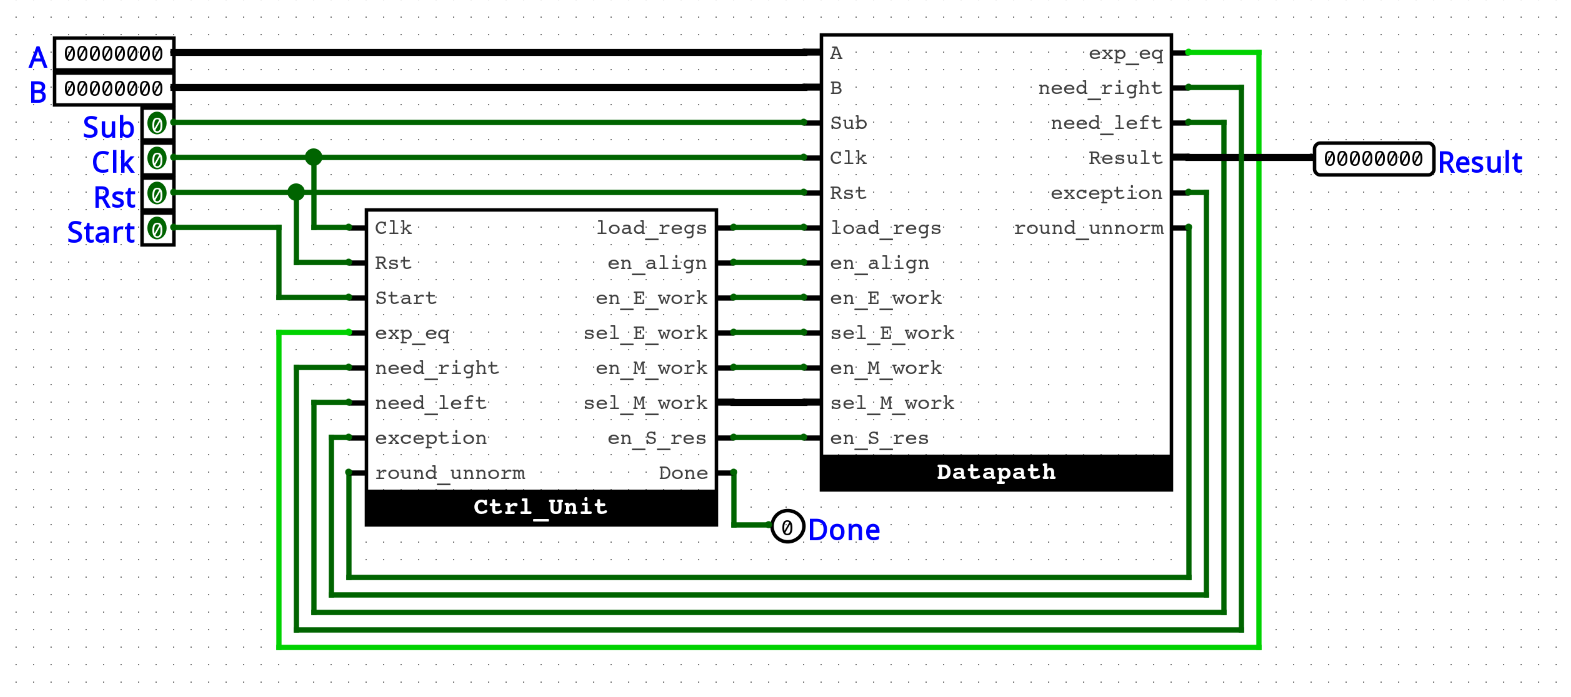
\includegraphics[width=1.0\textwidth]{assets/main.png}
    \caption{مدار نهایی و سطح بالای سیستم (\lr{\code{main}}) در محیط لاجیسیم}
\end{figure}

\pagebreak

\section{اجرای آزمون}
برای اطمینان از صحت عملکرد سیستم طراحی شده، تست‌کیس‌های مختلفی بر روی مدار اجرا گردید. صحت اجرای تمامی آزمون‌ها و پاس شدن ارزیابی‌ها در اسکرین‌شات زیر از خروجی تست‌ها مشهود است.

\begin{figure}[H]
    \centering
    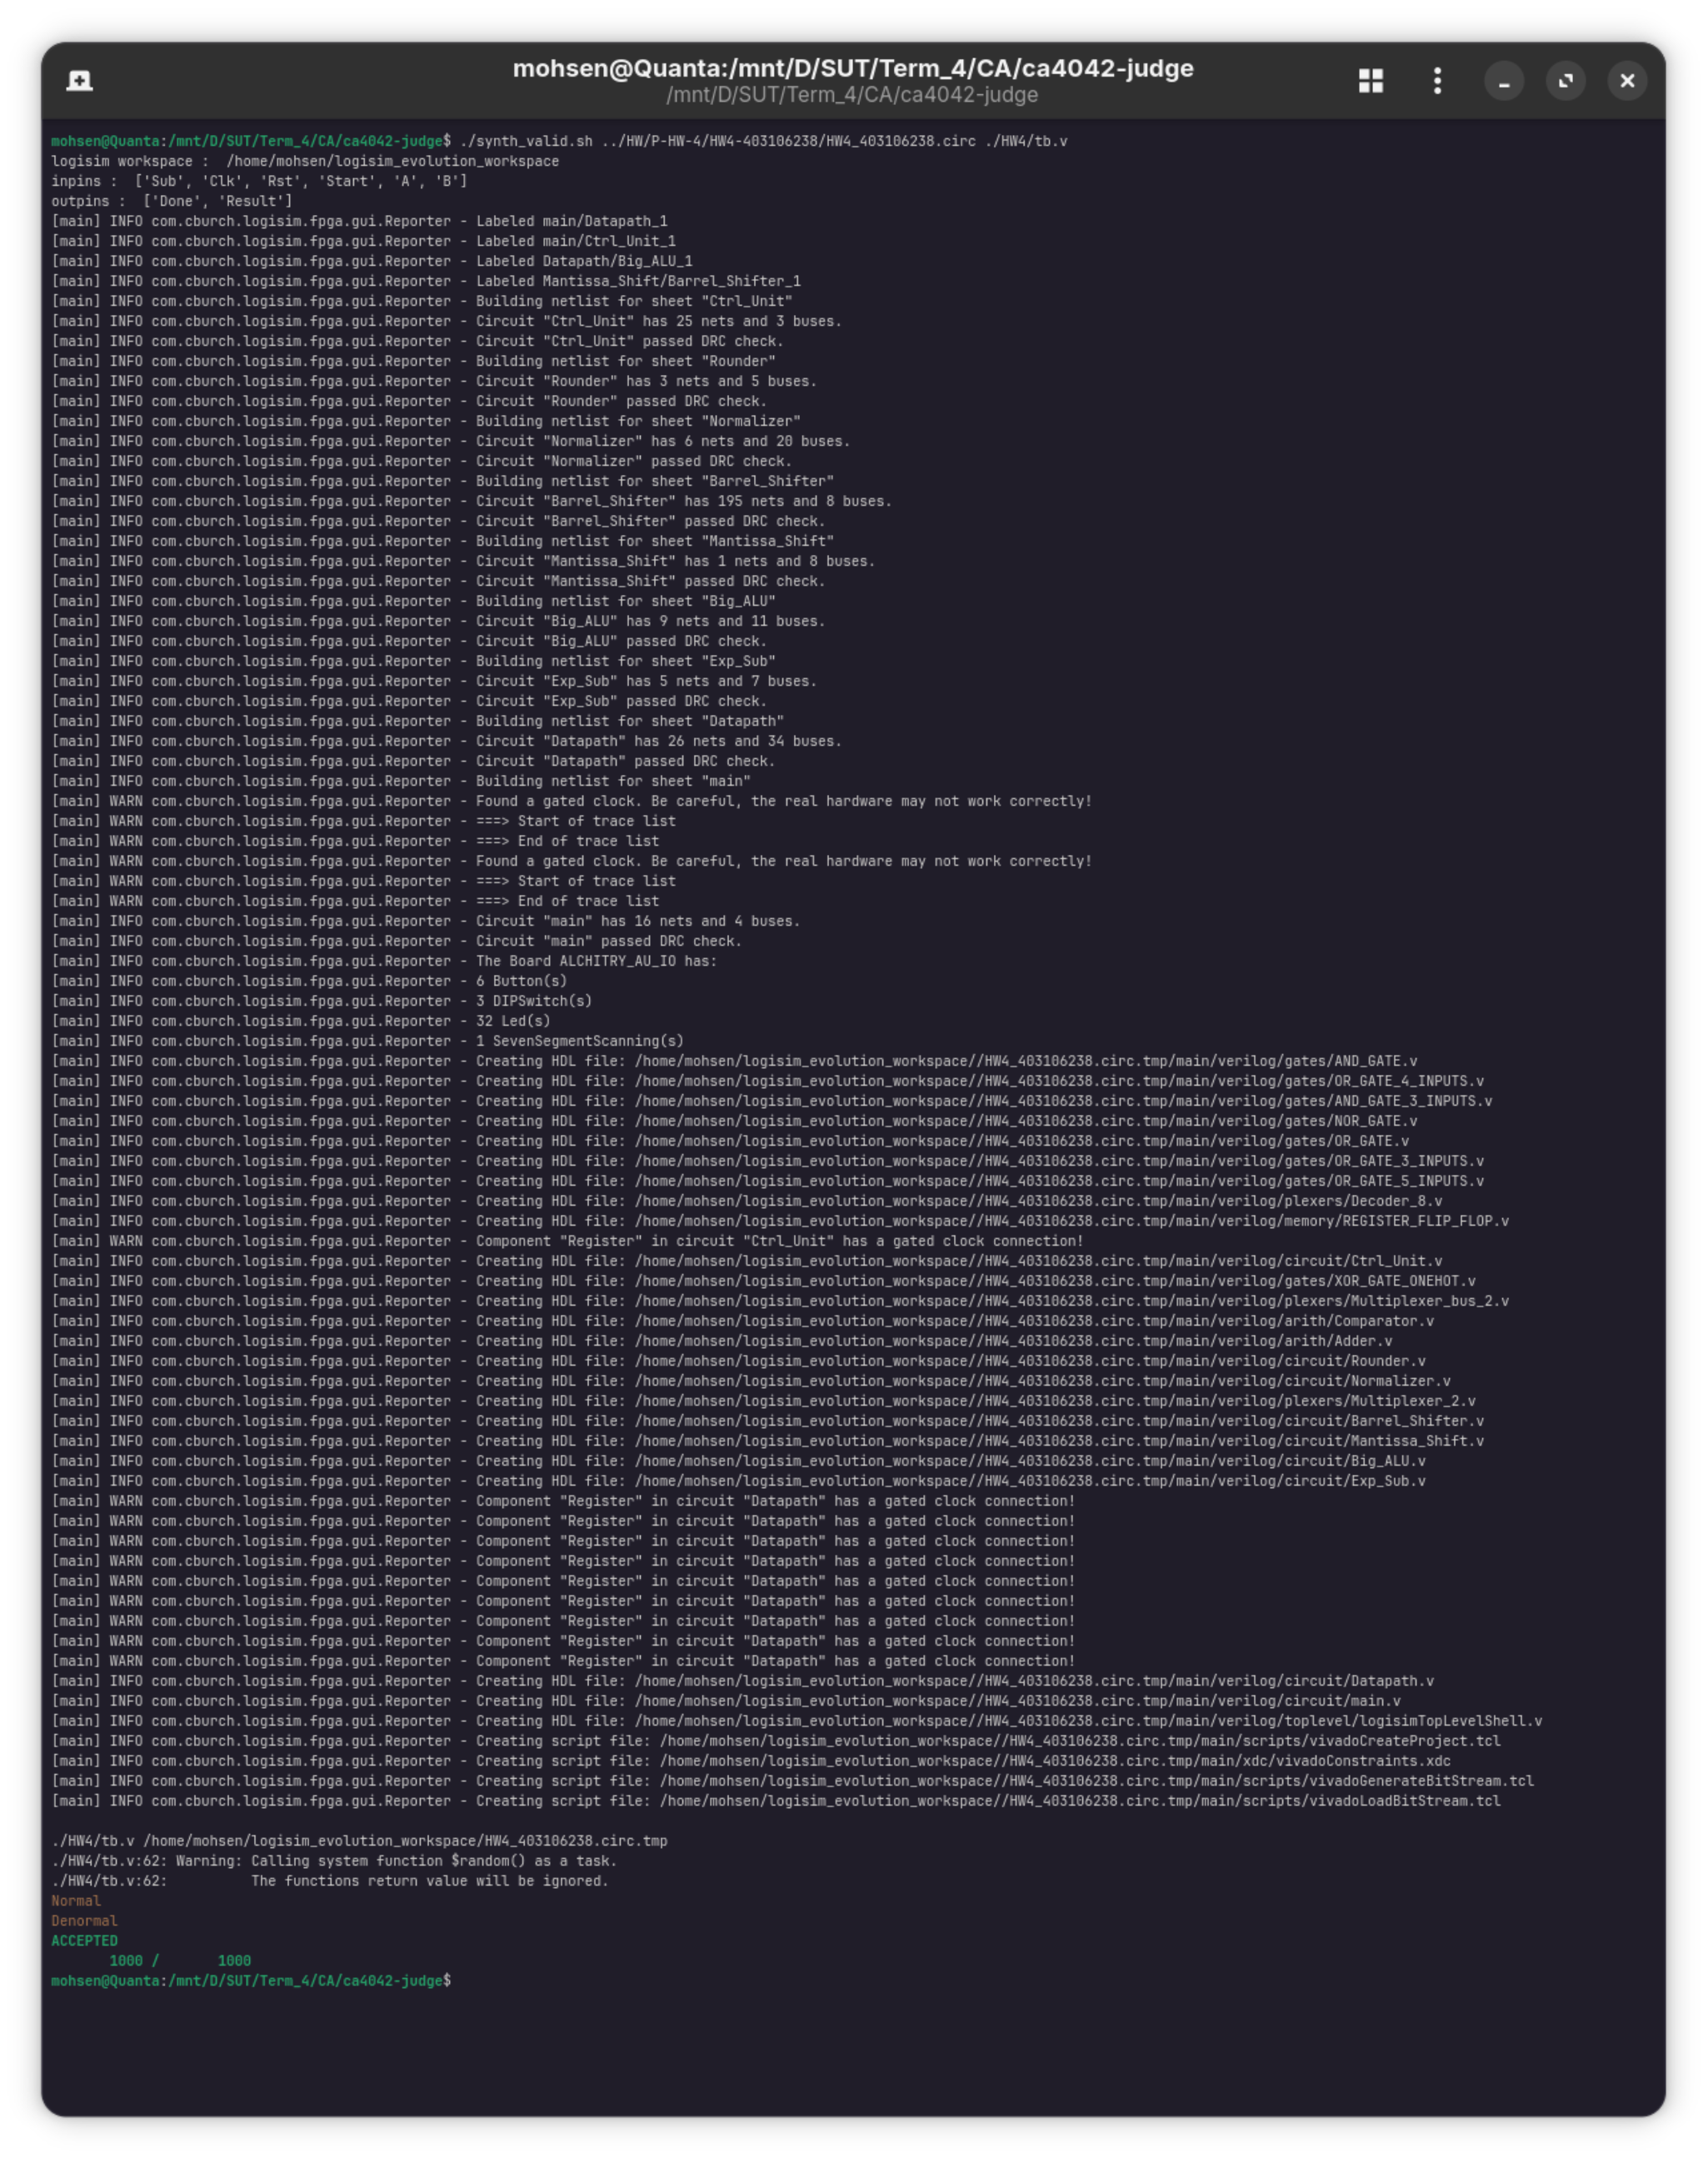
\includegraphics[width=1.0\textwidth]{assets/test_case.png}
    \caption{نتیجه اجرای موفقیت‌آمیز تست‌کیس‌های مدار}
\end{figure}